\documentclass[fleqn,10pt]{wlscirep}
\usepackage[utf8]{inputenc}
\usepackage[T1]{fontenc}
\title{BrainParc: Progressive Framework for Lifespan Brain Region Parcellation: Towards Comprehensive Understanding of Development and Aging}
%\title{BrainParc: Fully Automatic Progressive Brain Region Parcellation from T1w Image}
\author[1,2]{Jiameng Liu}
\author[1,2,3,4]{Dinggang Shen}
\affil[1]{School of Biomedical Engineering, ShanghaiTech University, Shanghai, China}
\affil[2]{State Key Laboratory of Advanced Medical Materials and Devices, ShanghaiTech University, Shanghai, China}
\affil[3]{Shanghai United Imaging Intelligence Co., Ltd., Shanghai, China}
\affil[4]{Shanghai Clinical Research and Trial Center, Shanghai, China}

%\keywords{Keyword1, Keyword2, Keyword3}
\keywords{Brain Region Parcellation, Progressive Segmentation, Keyword3}
\begin{abstract}
    A persistent challenge in automatic brain region parcellation from structural MR images in the literature is how to address the issue of generalization and robustness amidst substantial \textit{variations in intensity} caused by innate brain maturation and MR scanner manufacturers. Conventional methods for brain region parcellation are often sensitive to varying image contrast; even within the same individual scanned on different MR manufacturers or ages, performance tends to degrade across different scanners and ages. In this work, to address the issues mentioned above, we present a brain region parcellation (UniParc) framework, the first fully automatic segmentation model designed to handle the changes in intensity contrast across the lifespan of the human brain. Notably, UniSeg adopts a cascaded coarse-to-fine brain region parcellation framework that capitalizes on hierarchical, intensity-agnostic image representations (\textit{i.e.}, edge, boundary, and tissue) to effectively address the inherent intensity variation issues. UniParc is trained on the largest dataset to date, comprising over 20k T1w image samples spanning ages from 0-100 years, and sourced from diverse global populations (including variations in race, age, and disease status). Consequently, UniParc can automatically and accurately segment T1w brain images from a wide array of target domains without requiring fine-turning, accomplishing this task within two minutes. This capability streamlines the analysis of vast brain data, facilitating efficient research and clinical applications. Extensive experimentation on both internal and external testing datasets consistently demonstrates the superior performance and broad applicability of our proposed UniParc framework.
\end{abstract}

\begin{document}

\flushbottom
\maketitle



\thispagestyle{empty}

\section*{Introduction}

\begin{figure}[t]
    \begin{center}
    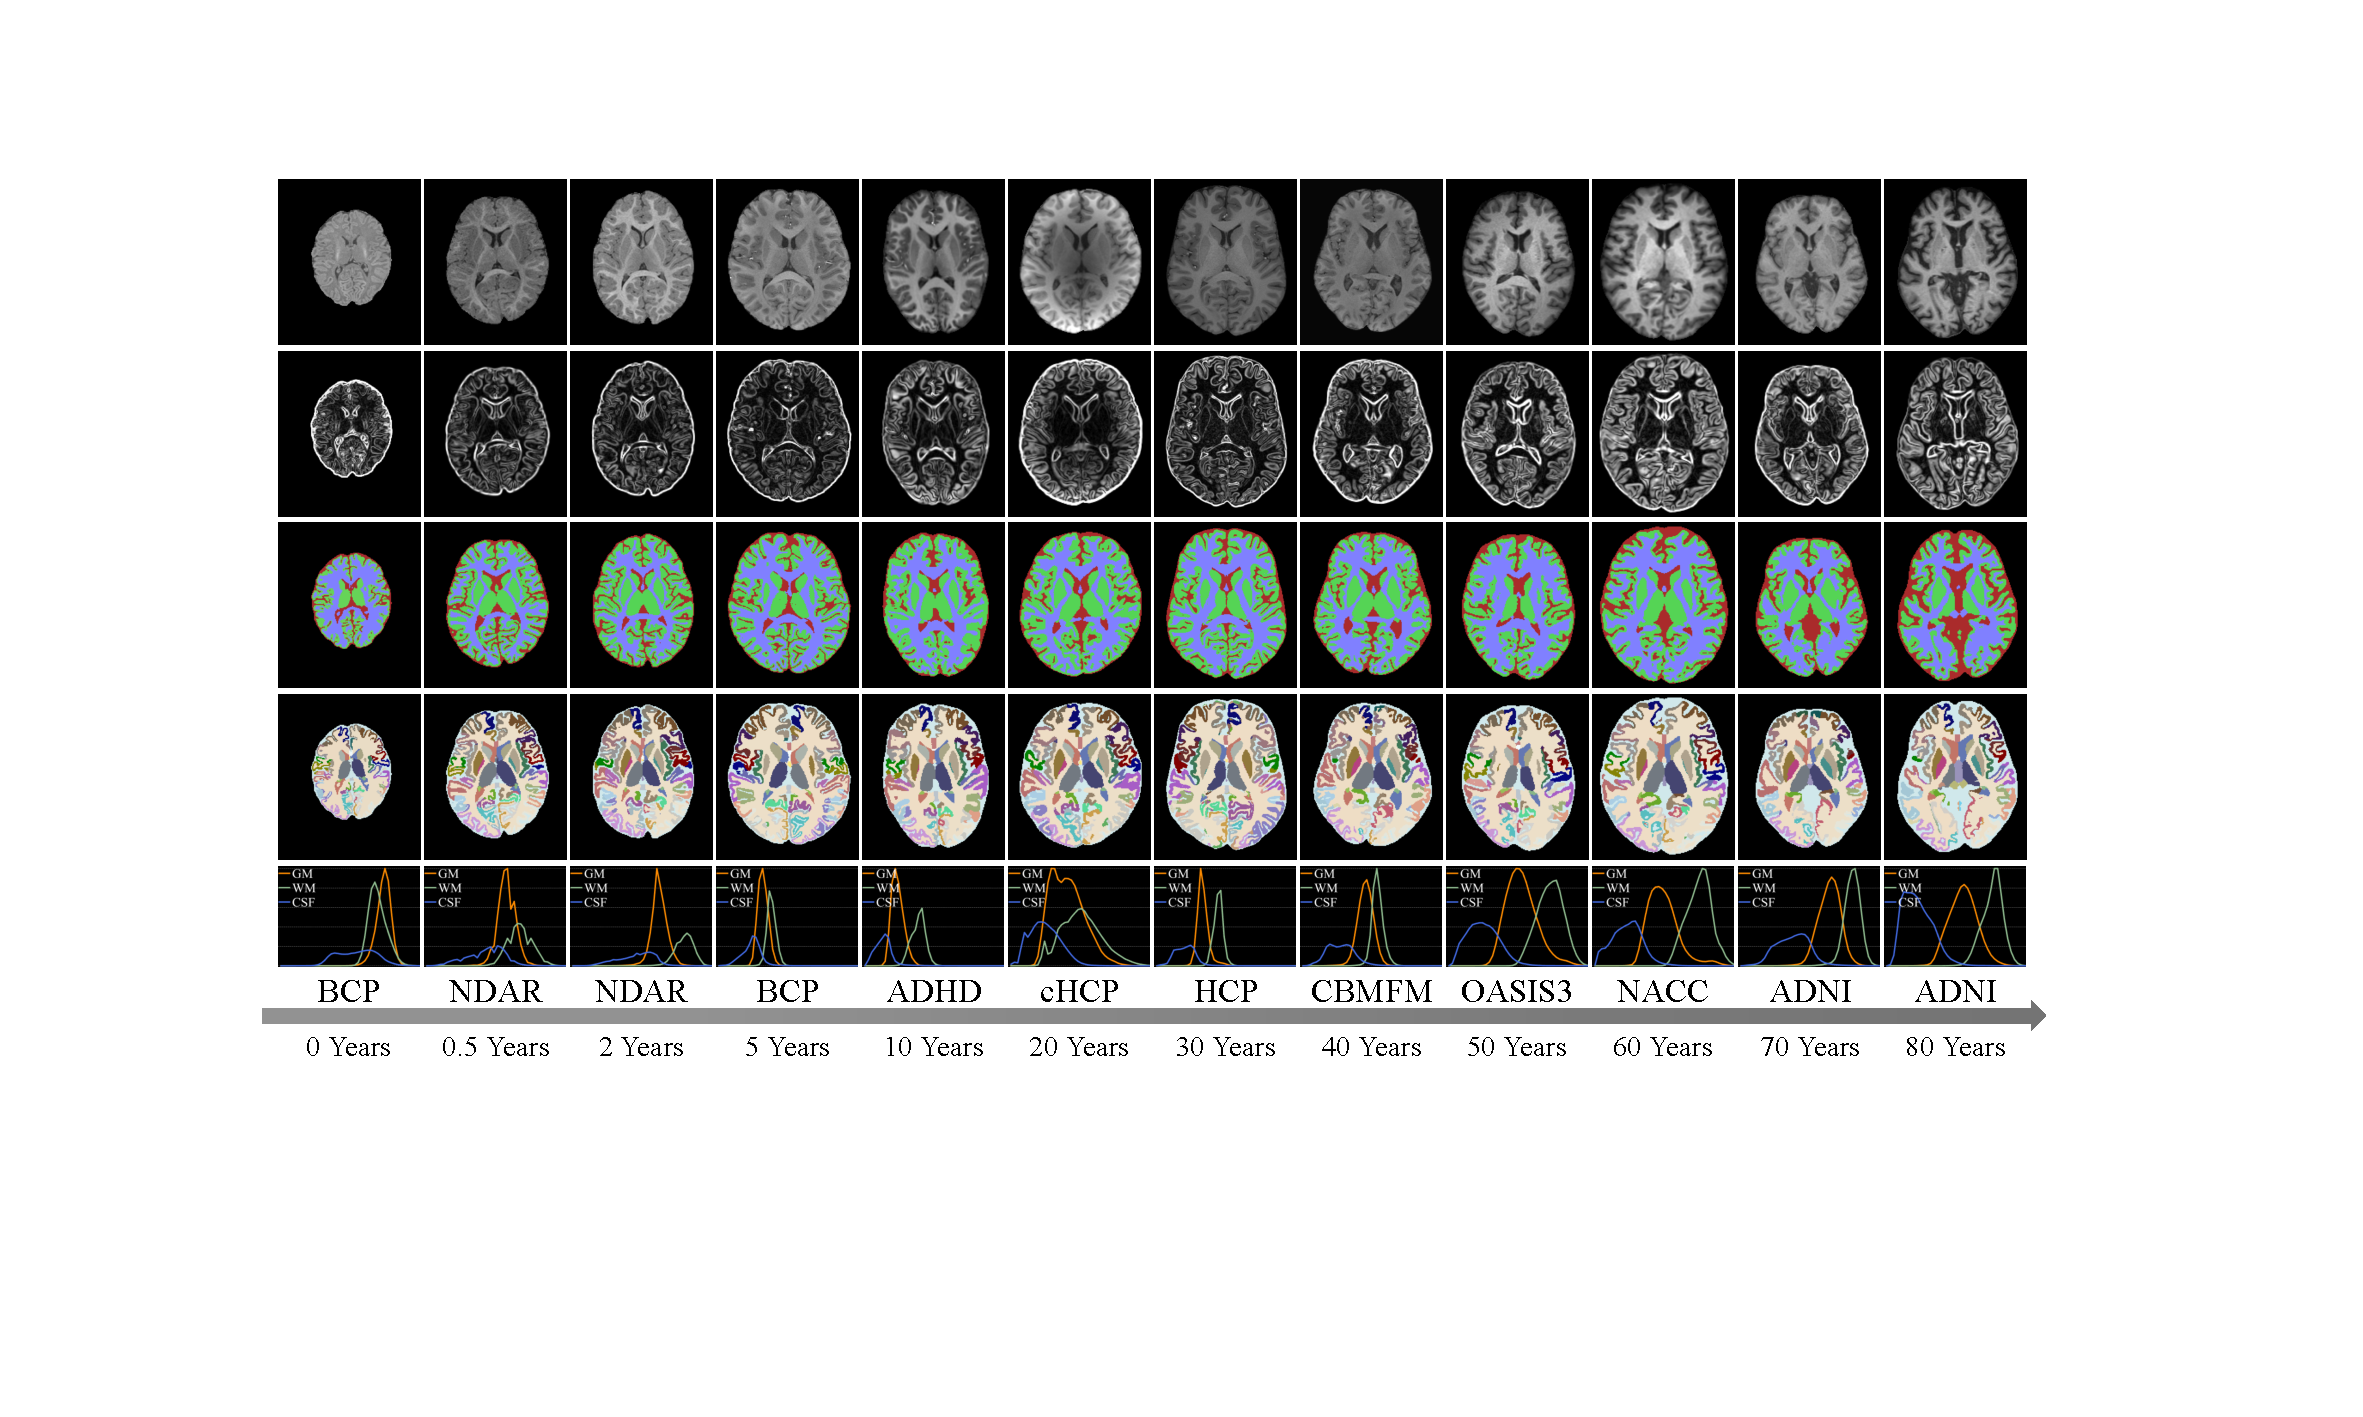
\includegraphics[width=0.98\textwidth]{./figure/data_sample.pdf}
    \caption{Representative intensity appearance across human brain development periods. From left to right present the brain at 0, 0.5, 2, 5, 10, 20, 30, 40, 50, 60, 70, and 80 years old. From top to bottom, intensity data, corresponding edge maps, tissue maps, dk-struct maps, and intensity distributions of three tissues, respectively.} \label{fig:data_sample}
    \end{center}
\end{figure}


\begin{figure}[t]
    \begin{center}
    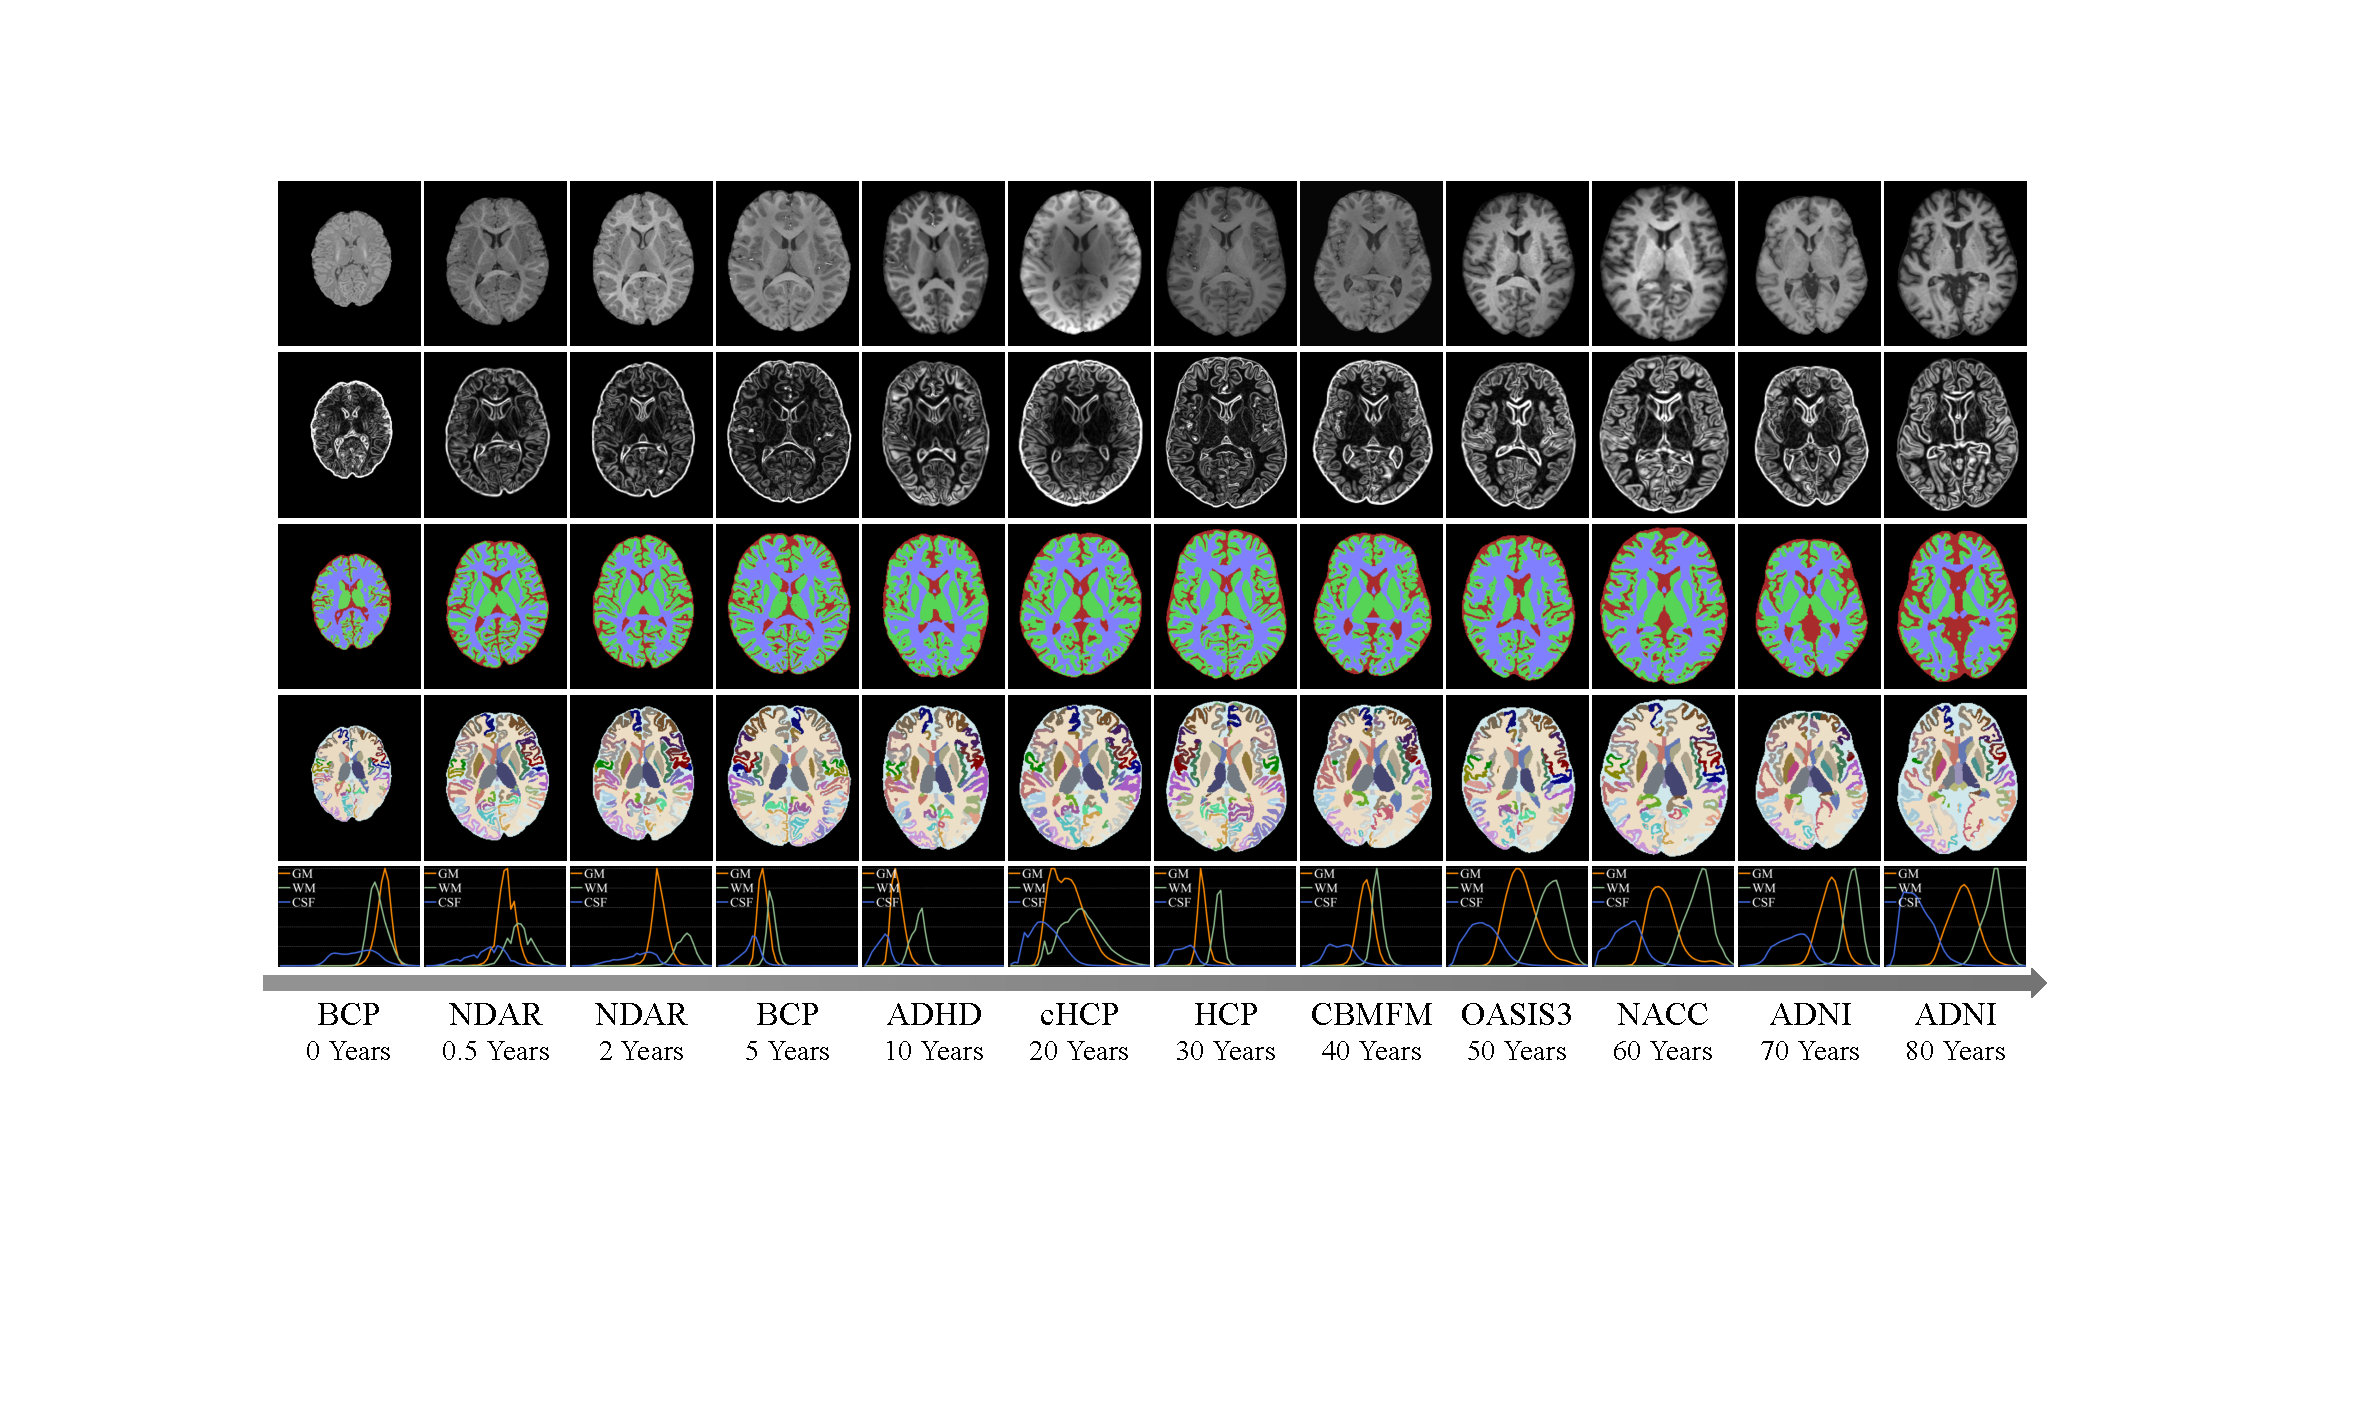
\includegraphics[width=0.98\textwidth]{./figure/data_sample_v1.pdf}
    \caption{Representative intensity appearance across human brain development periods. From left to right present the brain at 0, 0.5, 2, 5, 10, 20, 30, 40, 50, 60, 70, and 80 years old. From top to bottom, intensity data, corresponding edge maps, tissue maps, dk-struct maps, and intensity distributions of three tissues, respectively.} \label{fig:data_sample_v1}
    \end{center}
\end{figure}

\section*{Results}


\section*{Discussion}



\section*{Methods}



\bibliography{lifespanparc}



\section*{Acknowledgements (not compulsory)}

Acknowledgements should be brief, and should not include thanks to anonymous referees and editors, or effusive comments. Grant or contribution numbers may be acknowledged.

\section*{Author contributions statement}

Must include all authors, identified by initials, for example:
A.A. conceived the experiment(s),  A.A. and B.A. conducted the experiment(s), C.A. and D.A. analysed the results.  All authors reviewed the manuscript. 



\end{document}